% Created 2022-08-12 Fri 10:43
% Intended LaTeX compiler: pdflatex
\documentclass[11pt]{article}
\usepackage[utf8]{inputenc}
\usepackage[T1]{fontenc}
\usepackage{graphicx}
\usepackage{longtable}
\usepackage{wrapfig}
\usepackage{rotating}
\usepackage[normalem]{ulem}
\usepackage{amsmath}
\usepackage{amssymb}
\usepackage{capt-of}
\usepackage{hyperref}
\author{Andrin Bertschi}
\date{\today}
\title{Troubleshooting ad-free}
\hypersetup{
 pdfauthor={Andrin Bertschi},
 pdftitle={Troubleshooting ad-free},
 pdfkeywords={},
 pdfsubject={},
 pdfcreator={Emacs 27.2 (Org mode 9.6)}, 
 pdflang={English}}
\begin{document}

\maketitle
\tableofcontents



\section{About}
\label{sec:orge76b993}
This page describes common steps how to troubleshoot ad-free in case
ad blocking does not work.

\begin{itemize}
\item Pictures below are based on version v2.0. They may slightly change in later versions.

\item Landing page: \url{https://adfree.abertschi.ch}

\item Sourcecode: \url{https://github.com/abertschi/ad-free}
\end{itemize}

\section{Reinstall ad-free}
\label{sec:org1592811}
Remove and reinstall ad-free. Upon first usage you are asked to grant
notification access. Whether the notification service successfully
connected can be seen in settings (three dots in about fragment) in
the version segment. You can touch the \uline{notification service is
connected} / \uline{notification service is disconnected} text to launch
notification access settings to re-grant access.

\begin{figure}[htbp]
\centering
\includegraphics[width=200px]{./res/img-not-service-conn.jpg}
\caption{Notification service status}
\end{figure}

\section{Enable autostart}
\label{sec:org6369766}
Some flavors of Android support an autostart option. Go to Android app info
and enable auto start.

\begin{figure}[htbp]
\centering
\includegraphics[height=300px]{./res/app-info-autostart.jpg}
\caption{App info activity}
\end{figure}


\section{Disable battery saver}
\label{sec:org518a8ee}
Remove ad-free from the list of battery saved apps. This option can be
found in Android app info.

\begin{figure}[htbp]
\centering
\includegraphics[height=300px]{./res/app-info-battery-saver.jpg}
\caption{Battery saver options}
\end{figure}

\section{Enable always-on notifications}
\label{sec:org715fc82}
On some flavors of Android ad-free is being killed if the activity
runs in background. Go to ad-free settings (three dots in about
fragment) and enable always-on option. A foreground notification
should now appear in the notification drawer. This notification
appears as soon as the notification listener is connected an running.

\begin{figure}[htbp]
\centering
\includegraphics[height=300px]{./res/notification-always-on.jpg}
\caption{Always On Notification}
\end{figure}

\section{Avoiding false-positives}
\label{sec:orgfb24560}
A false-positive may be resolved with a new ad-detector. You can try to
screenshot the Spotify notification which caused the false-positive and file an
issue on Github.

Alternatively, we recommend to disable non-playback related notifications in the Android app spettings for Spotify.

\begin{figure}[htbp]
\centering
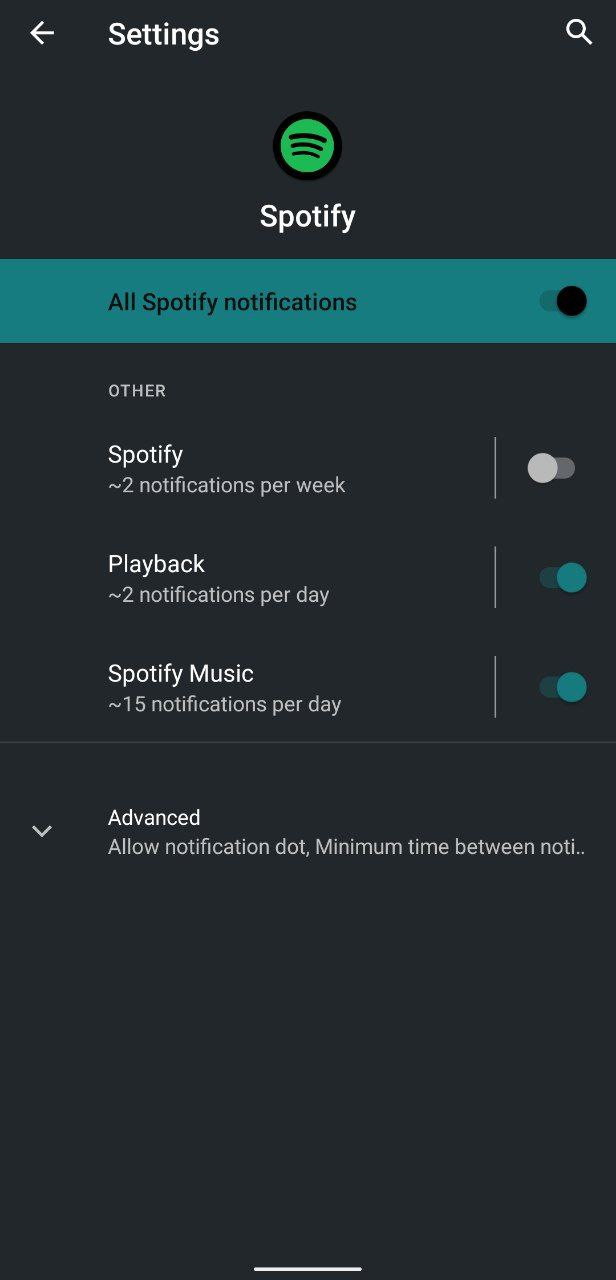
\includegraphics[height=300px]{./res/spotify-notifications.jpg}
\caption{Disable non-playback related notifications}
\end{figure}



\section{Advanced steps}
\label{sec:org60db236}
\subsection{Check if notification listener works}
\label{sec:org5d80e2f}
Enable developer mode in ad-free by clicking multiple times on the
title in the ad detectors screen. Go to ad-free settings (three dots)
/ ad detectors. Enable the detector \uline{Dummy global} which flags each
incoming notification as advertisement. If audio is not being blocked
then there is an issue with the notification listener. File an issue
on Github; \url{https://github.com/abertschi/ad-free/issues}.

\subsection{Record notifications for a new detector.}
\label{sec:orgdcbbebb}
Unlock developer mode as described above. Enable Spotify tracer and
submit the recording file as an issue on Github. The notification dump
can help adding support for new devices.


\section{Miscellaneous}
\label{sec:org3fdcc2a}
\subsection{Issues with Bluetooth Headphones}
\label{sec:org24ac2da}
See \url{https://github.com/abertschi/ad-free/issues/64} for troubleshooting steps.
\end{document}
